% % % % % % % %  MDT UFSM 2015  % % % % % % % % 
%% Arquivo base para o documento - ver. 1.08 %%
% % % % % % % % % % % % % % % % % % % % % % % % 


% % % OPCOES DE COMPILACAO
% % % PAGINACAO
% % % PAGINACAO SIMPLES (FRENTE): PARA TRABALHOS COM MENOS DE 100 PAGINAS
\documentclass[oneside,openright,12pt]{ufsm_2015} %%%%% OPCAO PADRAO -> PAGINACAO SIMPLES. PARA TRABALHOS COM MAIS DE 100 PAGINAS COMENTE ESTA LINHA E DESCOMENTE A LINHA 
% % % % % % % % % % % % % % % % % % % % % % % % % % % % % % % % % % % % % % %
% PAGINACAO DUPLA (FRENTE E VERSO): PARA TRABALHOS COM MAIS DE 100 PAGINAS
% \documentclass[twoside,openright,12pt]{ufsm_2015}  %%%% PARA TRABALHOS COM MAIS DE 100 PAGINAS DESCOMENTE AQUI
% % % % % % % % % % % % % % % % % % % % % % % % % % % % % % % % % % % % %




% % % %  CODIFICACAO DO TEXTO 
% % % %  POR PADRAO USA-SE UTF8. PARA APLICAR A CODIFICACAO OESTE EUROPEU (ISO 8859-1) DESCOMENTE A LINHA ABAIXO. ELA ATIVA A OPCAO "latin1" DO PACOTE "inputenc"
% \oesteeuropeu
% % % % % % % % % % % 



% % % % % % % % PACOTES PESSOAIS % % % % % % % %  
\usepackage{lipsum}





% % % % % % % % DEFINICOES PESSOAIS % % % % % % % %







% % % % % % % % % % % % % % % % % % % % % % % % % % % % % % % % % % % % % % % % % % % 




% % % % % % % % % % % % % % % % % % % % % % % % % % % % % % % % % 
% % % % % % % % % % % % DADOS DO TRABALHO % % % % % % % % % % % % 
% % % % % % % % % % % % % % % % % % % % % % % % % % % % % % % % % 

% % % % % % % % % % INFORMACOES INSTITUCIONAIS % % % % % % % % % % 


% % CENTRO DE ENSINO DA UFSM
\centroensino{Centro de Ciências Naturais e Exatas}  %%% NOME POR EXTENSO
\centroensinosigla{CCNE}  %%% SIGLA

% % CURSO DA UFSM
\nivelensino{Pós-Graduação}  %%%%%%% NIVEL DE ENSINO 
\curso{Algum Curso}   %%%%% NOME POR EXTENSO
\ppg{PPGALGO}   %%%%%% SIGLA
\statuscurso{Programa}  %%%% STATUS= {Programa} ou {Curso}
% \EAD  %%%% para cursos EAD
% % % %  LOCAL DO CAMPUS OU POLO
\cidade{Santa Maria}
\estado{RS}


% % % % % % % % % % INFORMACOES DO AUTOR % % % % % % % % % % 
\author{Fulano de Tal}   %%%%% AUTOR DO TRABALHO
\sexo{M} %%%% SEXO DO AUTOR -> M=masculino   F=feminino (IMPORTANTE PARA AJUSTAR PAGINAS PRE-TEXTUAIS)
\grauensino{Doutorado}    %%%%%%%% GRAU DE ENSINO A SER CONCLUIDO
\grauobtido{Doutor}    %%%%% TITULO OBTIDO
\email{lalala@uhul.com}   %%%% E-MAIL PARA CATALOGRAFICA (COPYRIGHT) - OBRIGATORIO
\endereco{Rua das abobrinhas, n. 666} %%%% TELEFONE PARA CATALOGRAFICA (COPYRIGHT) (CAMPO OPICIONAL -- CASO NAO POSSUA OU NAO QUEIRA DIVULGAR COMENTE A LINHA)
\fone{11 2222 3333}   %%%% TELEFONE PARA CATALOGRAFICA (COPYRIGHT) FORMATO {11 2222 3333} (CAMPO OPICIONAL -- CASO NAO POSSUA OU NAO QUEIRA DIVULGAR COMENTE A LINHA)
\fax{11 2222 3333}   %%%% FAX PARA CATALOGRAFICA (COPYRIGHT) FORMATO {11 2222 3333} (CAMPO OPICIONAL -- CASO NAO POSSUA OU NAO QUEIRA DIVULGAR COMENTE A LINHA)


% % % % % % % % % % INFORMACOES DA BANCA % % % % % % % % % % 
% OBSERVACOES: O CAMPO ORIENTADOR EH OBRIGATORIO E NAO DEVE SER COMENTADO
% % % % % %    OS DEMAIS MEMBROS DA BANCA (COOREIENTADOR E DEMAIS PROFESSORES) QUANDO COMENTADOS NAO APARECEM NA FOLHA DE APROVACAO (O LAYOUT DA FOLHA DE APROVACAO ESTA PREPARADO PARA O ORIENTADOR E ATE MAIS 4 MEMBROS NA BANCA
\orientador{João da Silva}{Dr}{AAAA}{M}{P}  %%%INFORMACOES SOBRE ORIENTADOR: OS CAMPOS SAO:{NOME}{SIGLA DA TITULACAO}{SIGLA DA INSTITUICAO DE ORIGEM}{SEXO} M=masculino   F=feminino {PARTE DA BANCA?} P=presidente  M=Membro  N=Nao faz parte
\coorientador{Maria da Costa}{Dra}{AAAA}{F}{M} %%%INFORMACOES SOBRE CO-ORIENTADOR: OS CAMPOS SAO:{NOME}{SIGLA DA TITULACAO}{SIGLA DA INSTITUICAO DE ORIGEM}{SEXO} M=masculino   F=feminino {PARTE DA BANCA?} P=presidente  M=Membro  N=Nao faz parte
\bancaum{Banca Um}{Dr}{AAAA}{F}{M}  %%%INFORMACOES SOBRE PRIMEIRO NOME DA BANCA: OS CAMPOS SAO:{NOME}{SIGLA DA TITULACAO}{SIGLA DA INSTITUICAO DE ORIGEM}{SEXO} M=masculino   F=feminino {PARTE DA BANCA?} P=presidente  M=Membro  N=Nao faz parte
\bancadois{Banca Dois}{Dr}{BBBB}  %%%INFORMACOES SOBRE SEGUNDO NOME DA BANCA: OS CAMPOS SAO:{NOME}{SIGLA DA TITULACAO}{SIGLA DA INSTITUICAO DE ORIGEM}
% \bancatres{Banca Três}{Dra}{CCCC} %%%INFORMACOES SOBRE TERCEIRO NOME DA BANCA: OS CAMPOS SAO:{NOME}{SIGLA DA TITULACAO}{SIGLA DA INSTITUICAO DE ORIGEM}
% \bancaquatro{Banca Quatro}{Dr}{DDDD} %%%INFORMACOES SOBRE QUARTO NOME DA BANCA: OS CAMPOS SAO:{NOME}{SIGLA DA TITULACAO}{SIGLA DA INSTITUICAO DE ORIGEM}
% \bancacinco{Banca Cinco}{Dra}{EEEE} %%%INFORMACOES SOBRE QUARTO NOME DA BANCA: OS CAMPOS SAO:{NOME}{SIGLA DA TITULACAO}{SIGLA DA INSTITUICAO DE ORIGEM}
% \supervisor{Al Paccino}{Dr}{MAFIA}{M}{N} %%%INFORMACOES SOBRE SUPERVISOR (indicado para estagios): OS CAMPOS SAO:{NOME}{SIGLA DA TITULACAO}{SIGLA DA INSTITUICAO DE ORIGEM}{SEXO} M=masculino   F=feminino {PARTE DA BANCA?} P=Presidente  M=Membro  N=Nao faz parte



% % % % % % % % % % REALIZACAO POR VIDEO CONFERENCIA (MEMORANDO 04/2016 BIBLIOTECA CENTRAL UFSM)
\videoconferencia % % % % QUANDO O ACADEMICO DEFENDE POR VIDEO CONFERENCIA (PERMITIDO PELO ARTIGO 82 DO REGIMENTO GERAL DA PRPGP/UFSM). PARA DEFESAS NAS QUAIS O ACADEMICO ESTA PRESENTE COMENTE ESTA LINHA
% % % % QUANDO UM DOS MEMBROS DA BANCA PARTICIPA POR VIDEO CONFERENCIA INDICAR O MEMBRO DE ACORDO COM A LISTA ABAIXO. CASO CONTRARIO MANTER A PALAVRA "NAO". SAO PERMITIDOS, PELO REGIMENTO PRGPGP (ARTIGO 83) ATE 2 MEMBROS 
\videoconferenciabancap{1}  %%%% PRIMEIRO MEMBRO
\videoconferenciabancas{NAO}  %%%%% SEGUNDO MEMBRO
% % O > ORIENTADOR
% % CO > COORIENTADOR% % % % QUANDO UM DOS MEMBROS DA BANCA PARTICIPA POR VIDEO CONFERENCIA INDICAR O MEMBRO DE ACORDO COM A LISTA ABAIXO. CASO CONTRARIO MANTER A PALAVRA "NAO". SAO PERMITIDOS, PELO REGIMENTO PRGPGP ATE 2 MEMBROS.
% % 1 > BANCA UM
% % 2 > BANCA DOIS
% % 3 > BANCA TRÊS
% % 4 > BANCA QUATRO
% % 5 > BANCA CINCO
% % S > SUPERVISOR
% % % % % % % % % % % % % % % % % % % % % % % % % % % % % % % % % % % % 



% % % % % % % % % % INFORMACOES SOBRE O TRABALHO % % % % % % % % % %
% % % %  TITULO DO TRABALHO
\titulo{Título do trabalho em português com no máximo três linhas} %% NAO EH NECESSARIO CAPITALIZAR
% % % %  TITULO DO TRABALHO EM INGLES
\englishtitle{Título do trabalho em inglês com no máximo três linhas}  %% NAO EH NECESSARIO CAPITALIZAR
% % % AREA DE CONCENTRACAO DO TRABALHO (CNPQ)
\areaconcentracao{Área de concentração do CNPq}
% % % TIPO DE TRABALHO - MANTER APENAS UMA LINHA DESCOMENTADA
\tese  %% Tese de <nivel de ensino>
% \qualificacao %% Exame de Qualificação de <nivel de ensino>
% \dissertacao %% Dissertacao de <nivel de ensino>
% \monografia %% Monografia
% \monografiag  %% Monografia (nao exibe area de concentracao)
% \tf  %% Trabalho Final de <nivel de ensino>
% \tfg  %% Trabalho Final de Graduacao (nao exibe area de concentracao)
% \tcc  %% Trabalho de Conclusao de Curso
% \tccg  %% Trabalho de Conclusao de Curso (nao exibe area de concentracao)
% \relatorio  %% Relatório de Estágio (nao exibe area de concentracao)
% \generico   %%% Alternativa para aqueles cursos que nao recebem o titulo de bacharel ou licenciado. Ex: engenharia, arquitetura, etc... Os campos abaixo tambem devem ser preenchidos
%     \tipogenerico{Tipo de trabalho em português}
%     \tipogenericoen{Tipo de trabalho em inglês}
%     \concordagenerico{o}
%     \graugenerico{Engenheiro Eletricista}
% % % DATA DA DEFESA 
\data{15}{12}{2011} %% FORMATO {DD}{MM}{AAAA}



% % % % %  ALGUMAS ENTRADAS PRE-TEXTUAIS
% % % % CASO NAO QUEIRA UTILIZA-LAS COMENTE A LINHA DE COMANDO
% % % EPIGRAFE
% \epigrafe{Winter is coming!}{Família Stark} %ESTRUTURA DE CAMPOS -> {Texto}{Autor}
% % % DEDICATORIA
% \dedicatoria{Aos que virão depois de nós}
% % % %  AGRADECIMENTOS
% \agradecimentos{A mim!}

% % % % %  RESUMO E PALAVRAS CHAVE DO RESUMO - OBRIGATORIO PARA MDT-UFSM
\resumo{
% \singlespacing
Escreva seu resumo aqui! Você pode digitá-lo diretamente neste arquivo ou usar o comando input. O resumo deve ter apenas uma página, desde o cabeçalho até as palavras chave. Caso seu resumo seja maior, use comandos para diminuir espaçamento e fonte (até um mínimo de 10pt) no texto. Você pode reduzir o espaçamento do texto removendo comentário da primeira linha deste campo: comando singlespacing. Segundo a MDT, é preciso que os resumos tenham, no máximo, 250 palavras para trabalhos de conclusão de curso de graduação, pós-graduação e iniciação científica e até 500 palavras para dissertações e teses.
}
\palavrachave{Palavra Chave 1. Palavra 2. Palavra 3. (...)}
% "... deverão constar, no mínimo, três palavras-chave, iniciadas em
% letras maiúsculas, cada termo separado dos demais por ponto, e
% finalizadas também por ponto." MDT 2012

% % % % %  ABSTRACT E PALAVRAS CHAVE DO RESUMO - OBRIGATORIO PARA MDT-UFSM
\abstract{
Write your abstract here! As recomendações do resumo também se aplicam ao abstract.
}
\keywords{Keyword 1. Keyword 2. Keyword 3. (...)}


% % %  ATIVACAO DE LISTAS E PAGINAS ESPECIAIS
% % %  PARA QUE APARECAO NAO NO TEXTO DESCOMENTE A LINHA ABAIXO -> POR PADRAO TODAS ESTAO ATIVIDADAS

% % LISTA DE FIGURAS 
% \semfiguras   %%(QUANDO ATIVIDA NAO EXIBE A LISTA)
% % LISTA DE GRAFICOS 
% \semgraficos   %%(QUANDO ATIVIDA NAO EXIBE A LISTA)
% % LISTA DE ILUSTRACOES 
% \semilustracoes  %%(QUANDO ATIVIDA NAO EXIBE A LISTA)
% % LISTA DE TABELAS 
% \semtabelas   %%(QUANDO ATIVIDA NAO EXIBE A LISTA)
% % LISTA DE QUADROS 
% \semquadros   %%(QUANDO ATIVIDA NAO EXIBE A LISTA)
% % LISTA DE APENDICES 
% \semapendices  %%(QUANDO ATIVIDA NAO EXIBE A LISTA)
% LISTA DE ANEXOS 
% \semanexos   %%(QUANDO ATIVIDA NAO EXIBE A LISTA)



% % % %  LISTA DE ABREVIATURAS E SIGLAS
%%%%%%%% OBS: O espaco entre colchetes \item[] e um ambiente matematico
%%%%%%%% para não utilizar comente as linhas abaixo.
\siglamax{SIGLAMAX} %%%% coloque aqui a maior sigla (indentacao)
\listadeabreviaturasesiglas{
\item[SIGLA1]	Nome Completo da Sigla 1
\item[SIGLA2]	Nome Completo da Sigla 2
\item[SIGLAMAX]	Nome Completo da Sigla MAX
}

% % % %  LISTA DE SIMBOLOS
%%%%%%%% OBS: O espaco entre colchetes \item[] e um ambiente matematico
%%%%%%%% para não utilizar comente as linhas abaixo.
\simbolomax{(Re)2} %%%% coloque aqui o maior simbolo (indentacao)
\listadesimbolos{
\item[u_*]	Escala de velocidade de fricção	
\item[w_*]	Escala de velocidade convectiva
\item[(Re)^2]	Maior simbolo da lista
}


% % % FICHA CATALOGRAFICA
% \semcatalografica  %%%%  (QUANDO ATIVIDA NAO EXIBE A FICHA CATALOGRAFICA NECESSITA DO ARQUIVO DA FICHA: ficha_catalografica.pdf
% % % A FICHA CATALOGRAFICA FORNECIDA PELA UFSM EH UM PDF DO TAMANHO A4
% % % EH POSSIVEL GERA-LA NO SITE http://cascavel.ufsm.br/ficha_catalografica/
% % % OS COMANDOS ABAIXO DEFINEM AS MARGENS PARA CORTAR A FICHA FORNECIDA E COLOCA-LA COMO UMA FIGURA NO DOCUMENTO LATEX
\margemesquerda{4}   %%%% CORTE DE MARGEM ESQUERDA EM CM
\margemdireita{1.5}   %%%% CORTE DE MARGEM DIREITA EM CM
\margemsuperior{17}  %%%% CORTE DE MARGEM SUPERIOR EM CM
\margeminferior{3} %%%% CORTE DE MARGEM INFERIOR EM CM
% % %  DICA: IMPRIMA UMA COPIA DA FICHA CATALOGRAFICA E FACA A MEDIDA DAS MARGENS!





% % FOLHA DE ERRADA (versao rudimentar...pode ser aprimorado)
% % para não utilizar comente as linhas abaixo.
% % deve ser preenchida como um ambiente tabular de quatro colunas:
% % pagina & linha & onde se le & leia-a se \\
\errata{
10   &    10    & errado   & certo \\
\hline
12    &    5     & errado com um texto mais longo & certo agora com um texto mais longo\\
\hline
13   &    3    & $x^2$   & $2x$\\
}
% % % % % % % % % % % % % % % % % % % % % % % % % % % % % % % % % % % % % % % % % % % % % % 


% % % % % % % % % % % % % % % % % % % % % % % % % % % % % % % % % % % % % % 
% % % % % % % % % % % %  OPCOES DE FORMATACAO % % % % % % % % % % % % % % %
% % % % % % % % % % % % % % % % % % % % % % % % % % % % % % % % % % % % % % 
% % % CAPITULO: por padrao alinhado a esquerda. Para ativar alinhamento centralizado descomente o comando abaixo

% \centralizado  %%%% <<< centraliza todos os capitulos

% % % % % % % % % % % % % % % % % % % % % % % % % % % % % % % % % % % % % %
% % % FONTES: descomente uma das opcoes. caso nenhuma seja ativada a clase usara a fonte padrao do latex

%% helvetica
\usepackage[scaled]{helvet}
\renewcommand*\familydefault{\sfdefault}

%% arial
% \renewcommand{\rmdefault}{phv} % Arial
% \renewcommand{\sfdefault}{phv} % Arial

%%times
% \usepackage{mathptmx}

% % % % % % % % % % % % % % % % % % % % % % % % % % % % % % % % % % % % % % 
% % % % % % % % % % % % % % % % % % % % % % % % % % % % % % % % % % % % % % 
% % % % % % % % % % % % % % % % % % % % % % % % % % % % % % % % % % % % % % 
% % % % % % % % % % % % % % % % % % % % % % % % % % % % % % % % % % % % % % 


% % % % % % % % % % % % % % % % % % % % % % % % % % % % % % % % % % % % % % 
% % % % % % % % % % % % % % % % % % % % % % % % % % % % % % % % % % % % % % 
% % % % % % % % % % % %  INICIO DO DOCUMENTO  % % % % % % % % % % % % % % %
% % % % % % % % % % % % % % % % % % % % % % % % % % % % % % % % % % % % % % 
% % % % % % % % % % % % % % % % % % % % % % % % % % % % % % % % % % % % % %


\begin{document}



% % % % % % % % % % % % % % % % % % % % % % % % % % % % % % % % % % % % % % 
\pretextual  %%%% GERA AS PAGINAS PRE-TEXTUAIS   
% % % % % % % % % % % % % % % % % % % % % % % % % % % % % % % % % % % % % % 

% % % % % % % % % % % % % % % % % % % % % % % % % % % % % % % % % % % % % % 
% % % % % CORPO DO TRABALHO - INCLUA OS SEUS TEXTOS AQUI
% % % % % SUGESTAO -> UTILIZE ARQUIVOS EXTERNOS A PARTIR DO COMANDO \input
% % % % % % % % % % % % % % % % % % % % % % % % % % % % % % % % % % % % % % 
% % % % % % % % % % INICIO DAS PAGINAS TEXTUAIS % % % % % % % % % % % % % % 
% % % % % % % % % % % % % % % % % % % % % % % % % % % % % % % % % % % % % % 

\chapter{Introdução}
\par Insira aqui a introdução!!!

\lipsum[1-5]



\chapter{Algumas notas sobre bibliografia}


\par O arquivo \textit{referencias.bib} é o nome padrão das referências para este modelo. Para alterá-lo modifique o argumento entre chaves na definição de bibliografia.


   \section{Modelos de citação}
      \par No arquivo modelo de referências, também existem alguns exemplos de diferentes classes de citações. Todas elas podem ser usadas com o \textit{$\backslash$cite$\{$label$\}$} ou \textit{$\backslash$citeonline$\{$label$\}$}, dependendo da forma de citação\footnote{Este é um teste de nota de rodapé}.

	\par Além disso, pode-se incluir obras na bibliografia que nortearam o trabalho mesmo que elas não apareçam diretamente no texto, utilizando o comando \textit{$\backslash$nocite$\{$label$\}$}. Além disso, pode-se citar vários trabalhos em conjunto, por exemplo:
	
	\begin{center}\rule{0.5\textwidth}{1pt}\\$\backslash cite\{label1,label2,label3,...\}$\end{center}

	\begin{verbatim}
	Os ventos do norte não movem moinhos \cite{tcc:mintegui2014, 
	diss:anabor2004, tese:anabor2008, livro:halliday28ed, 
	livro:fedorova:v1, site:amsglo:fog}.
	\end{verbatim}
	    
	\par Os ventos do norte\footnote{Este é um teste de nota de rodapé} não movem moinhos \cite{tcc:mintegui2014,diss:anabor2004,tese:anabor2008,livro:halliday28ed,livro:fedorova:v1,site:amsglo:fog}.
        
        \begin{center}\rule{0.5\textwidth}{1pt}\\$\backslash citeonline\{label1,label2,label3,...\}$\end{center}
        
	\begin{verbatim}
	Segundo \citeonline{cap:livro:djuric1994, livro:aris1989, 
	livro:cotton1989, cap:livro:wyngaard1981, livro:fedorova:v1, 
	artigo:fujita1981,puhalesBLT2010,artigo:janjic2002,
	cbmet:anabor2012,site:wrfhome}, os ventos do norte não movem moinhos.
	\end{verbatim}
            
        \par Segundo \citeonline{cap:livro:djuric1994, livro:aris1989, livro:cotton1989, cap:livro:wyngaard1981, livro:fedorova:v1, artigo:fujita1981,puhalesBLT2010,artigo:janjic2002,cbmet:anabor2012,site:wrfhome}, os ventos\footnote{Este é um teste de nota de rodapé} do norte não movem moinhos.
        \begin{center}\rule{0.5\textwidth}{1pt}\end{center}   
         \par OBS: Trabalhos com mais de três autores aparecerão com a abreviatura ``et al'' no corpo do texto, porém todos os nomes da bibliografia (norma da UFSM que é definida nas opões do abntcite nas definições do arquivo). 
  
  \subsection{O comando \textit{apud}}

  \par A citação \textit{apud} ocorre quando você cita algum autor através de outra obra, sem ter consultado-a propriamente. Neste caso a citação é feita da seguinte forma:
  \begin{center}
  \rule{0.5\textwidth}{1pt}\\
  $\backslash apud\{material\_citado\_no\_material\_lido\}\{material\_lido\}$ \\
  \end{center}
\begin{verbatim}
Sobre a circulação geral da atmosfera pode-se dizer que os ventos do norte
não movem moinhos \apud{apud:richardson1922}{livro:monin:v1}.
\end{verbatim}
  
  Sobre a circulação geral da atmosfera pode-se dizer que os ventos do nortenão movem moinhos \apud{apud:richardson1922}{livro:monin:v1}.
\begin{center}\rule{0.5\textwidth}{1pt}\end{center}  
  \par Nesse caso, na bibliografia só constará a obra consultada e não aquele referenciada pela obra. Para que isso ocorra naturalmente, a obra consultada deve ser incluída normalmente no arquivo referencias.bib enquanto a obra referenciada indiretamente deve ser incluída com a opção \textit{@hidden}, conforme o modelo de referências\footnote{Isto é um teste de nota de rodapé}.

      \subsubsection{\textit{Apud on line}}

      
      \par O \textit{apudonline} se aplica da mesma maneira que o \textit{apud} descrito anteriormente. O termo \textit{on line} é alusivo ao \textit{$\backslash$citeonline$\{$label$\}$} definido no abntex. Nesse caso a citação é feita da seguinte forma:
      \begin{center}
      \rule{0.5\textwidth}{1pt}
            $\backslash apudonline\{material\_citado\_no\_material\_lido\}\{material\_lido\}$ \\
	    \end{center}

 \begin{verbatim}
Segundo \apudonline{apud:richardson1922}{livro:monin:v1}, os ventos do
norte não movem moinhos.
\end{verbatim}

            Segundo \apudonline{apud:richardson1922}{livro:monin:v1}, os ventos do norte não movem moinhos.

       \paragraph{Teste de seção quinária}
       
       \par Texto texto texto.
       
       
         \chapter{Tabelas, figuras, quadros, ilustrações e gráficos}
         
         \par Na MDT da UFSM há uma clara diferença entre tabelas e quadros, quanto a sua apresentação. Aqui, para inserir tabelas usa-se o ambiente tradicionalmente definido \textit{table}. A partir deste modelo simples:
        
         \begin{verbatim}
		\begin{table}[ht]
		\centering
		\caption{Modelo de tabela para MDT-UFSM.}
		\begin{tabular}{ c c c }
		\hline
		Abacate & Banana & Canela \\
		\hline
		21 & 34 & 56 \\
		-3 & 245 & 23 \\
		-25 & -0,57 & 2 \\
                \hline
                 \end{tabular}
		\fonte{Adaptado de \citeonline{livro:halliday28ed}.}
		\end{table}
	  \end{verbatim}
         
         \noindent resulta:
         
         \begin{table}[ht]
         \centering
         \caption{Modelo de tabela para MDT-UFSM.}
         \begin{tabular}{ c c c }
         \hline
         Abacate & Banana & Canela \\
         \hline
         21 & 34 & 56 \\
         -3 & 245 & 23 \\
         -25 & -0,57 & 2 \\
         \hline
         \end{tabular}
          \fonte{Adaptado de \citeonline{livro:halliday28ed}.}
         \end{table}
         
         \par Note que, adicionalmente, foi definido um comando novo: ``fonte''. Ele serve para indicar a fonte da tabela quando necessário, mas também pode ser usado em outros ambientes.
         
         \par Para inserir quadros foi criado um novo ambiente: ``quadro''. O ambiente ``quadro'' deve ser usado de forma semelhante a tabela, como o ambiente tabular. Contudo, neste caso, as linhas verticais e horizontais estão sempre presentes. Um exemplo simples é o seguinte: 
         
         
         \begin{verbatim}
	    \begin{quadro}
   	    \caption{Modelo de quadro para MTD-UFSM.}
	    \centering
	    \begin{tabular}{| c |c |c }
	    \hline
	    Abacate & Banana & Canela \\
	    \hline
	    21 & 34 & 56 \\
	    \hline
	    -3 & 245 & 23 \\
	    \hline
	    -25 & -0,57 & 2 \\
	    \hline
	    \end{tabular}
	    \fonte{Adaptado de \citeonline{livro:halliday28ed}.}
	    \end{quadro}
         \end{verbatim}
         
         \noindent resultando:
         
	    \begin{quadro}
	    \caption{Modelo de quadro para MTD-UFSM.}
	    \centering
	    \begin{tabular}{| c |c |c |}
	    \hline
	    Abacate & Banana & Canela \\
	    \hline
	    21 & 34 & 56 \\
	    \hline
	    -3 & 245 & 23 \\
	    \hline
	    -25 & -0,57 & 2 \\
	    \hline
	    \end{tabular}
    	    \fonte{Adaptado de \citeonline{livro:halliday28ed}.}
	    \end{quadro}
	    
	    
         \noindent Assim como para as tabelas, já está definida uma lista de quadros. Além disso, o comando ``fonte'' também pode ser usado aqui se necessário. Vale lembrar que, na MDT-UFSM, as legendas para figuras, tabelas, quadros, ilustrações e gráficos devem ser inseridas no topo da(o) mesma(o). A fonte sempre embaixo.
         
         \par As figuras devem ser inseridas com o ambiente padrão: \textit{figure}. Veja um exemplo simples:
         
         \begin{verbatim}
	    \begin{figure}[ht]
		\caption{\label{exepretex}Sequência dos elementros pré-testuais da MDT-UFSM.}
		\centering
		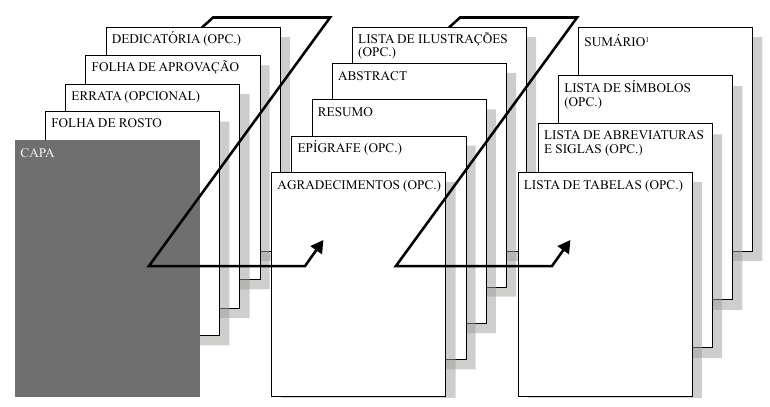
\includegraphics[width=0.6\textwidth]{figuras/pretextuais.png}
		\fonte{Adaptado de \citeonline{man:MDTUFSM2015}.}
	    \end{figure}
         \end{verbatim}
         
         \begin{figure}[ht]
     	    \caption{\label{exepretex}Sequência dos elementros pré-testuais da MDT-UFSM.}
	    \centering
	    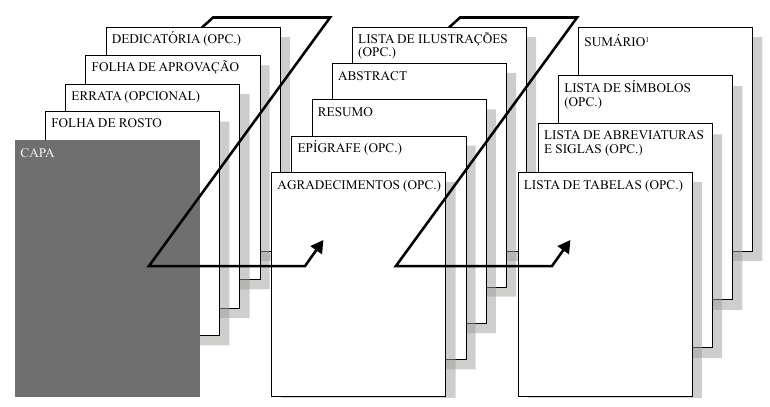
\includegraphics[width=0.6\textwidth]{figuras/pretextuais.png}
            \fonte{Adaptado de \citeonline{man:MDTUFSM2015}.}
         \end{figure}
        
	\par Para inserir ilustrações e gráficos, foram criados novos ambientes: ``ilustracao'' e ``grafico''. Estes ambientes são semelhantes ao ambiente ``figure'', porém geram sua própria lista. A seguir, exemplos da utilização nos novos ambientes.
	
	\begin{verbatim}
	    \begin{ilustracao}[ht]
		\caption{\label{exepretex1}Sequência dos elementros pré-testuais da MDT-UFSM}
                \centering
		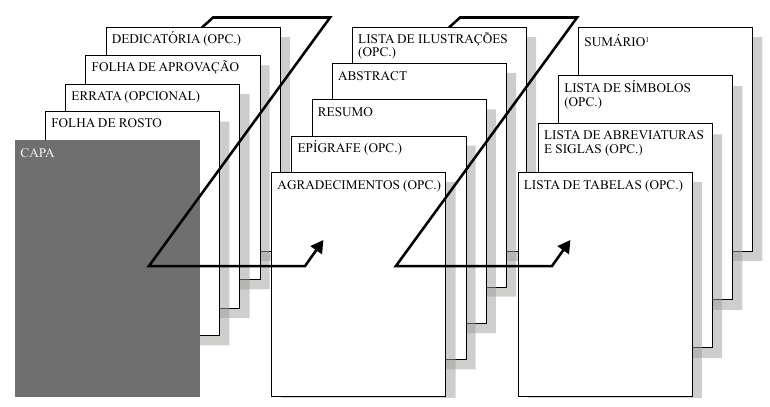
\includegraphics[width=0.6\textwidth]{figuras/pretextuais.png}
		\fonte{Adaptado de \citeonline{man:MDTUFSM2015}.}
	    \end{ilustracao}
         \end{verbatim}
         
         \begin{ilustracao}[ht]
     	    \caption{\label{exepretex1}Sequência dos elementros pré-testuais da MDT-UFSM.}
	    \centering
	    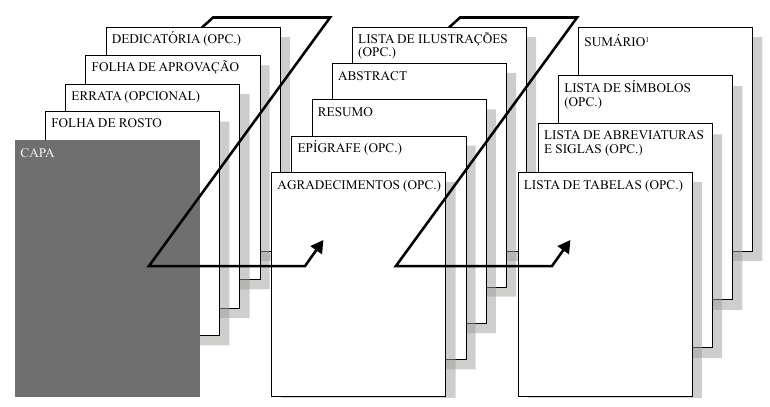
\includegraphics[width=0.6\textwidth]{figuras/pretextuais.png}
            \fonte{Adaptado de \citeonline{man:MDTUFSM2015}.}
         \end{ilustracao}
	
         
	\begin{verbatim}
	    \begin{grafico}[ht]
		\centering
		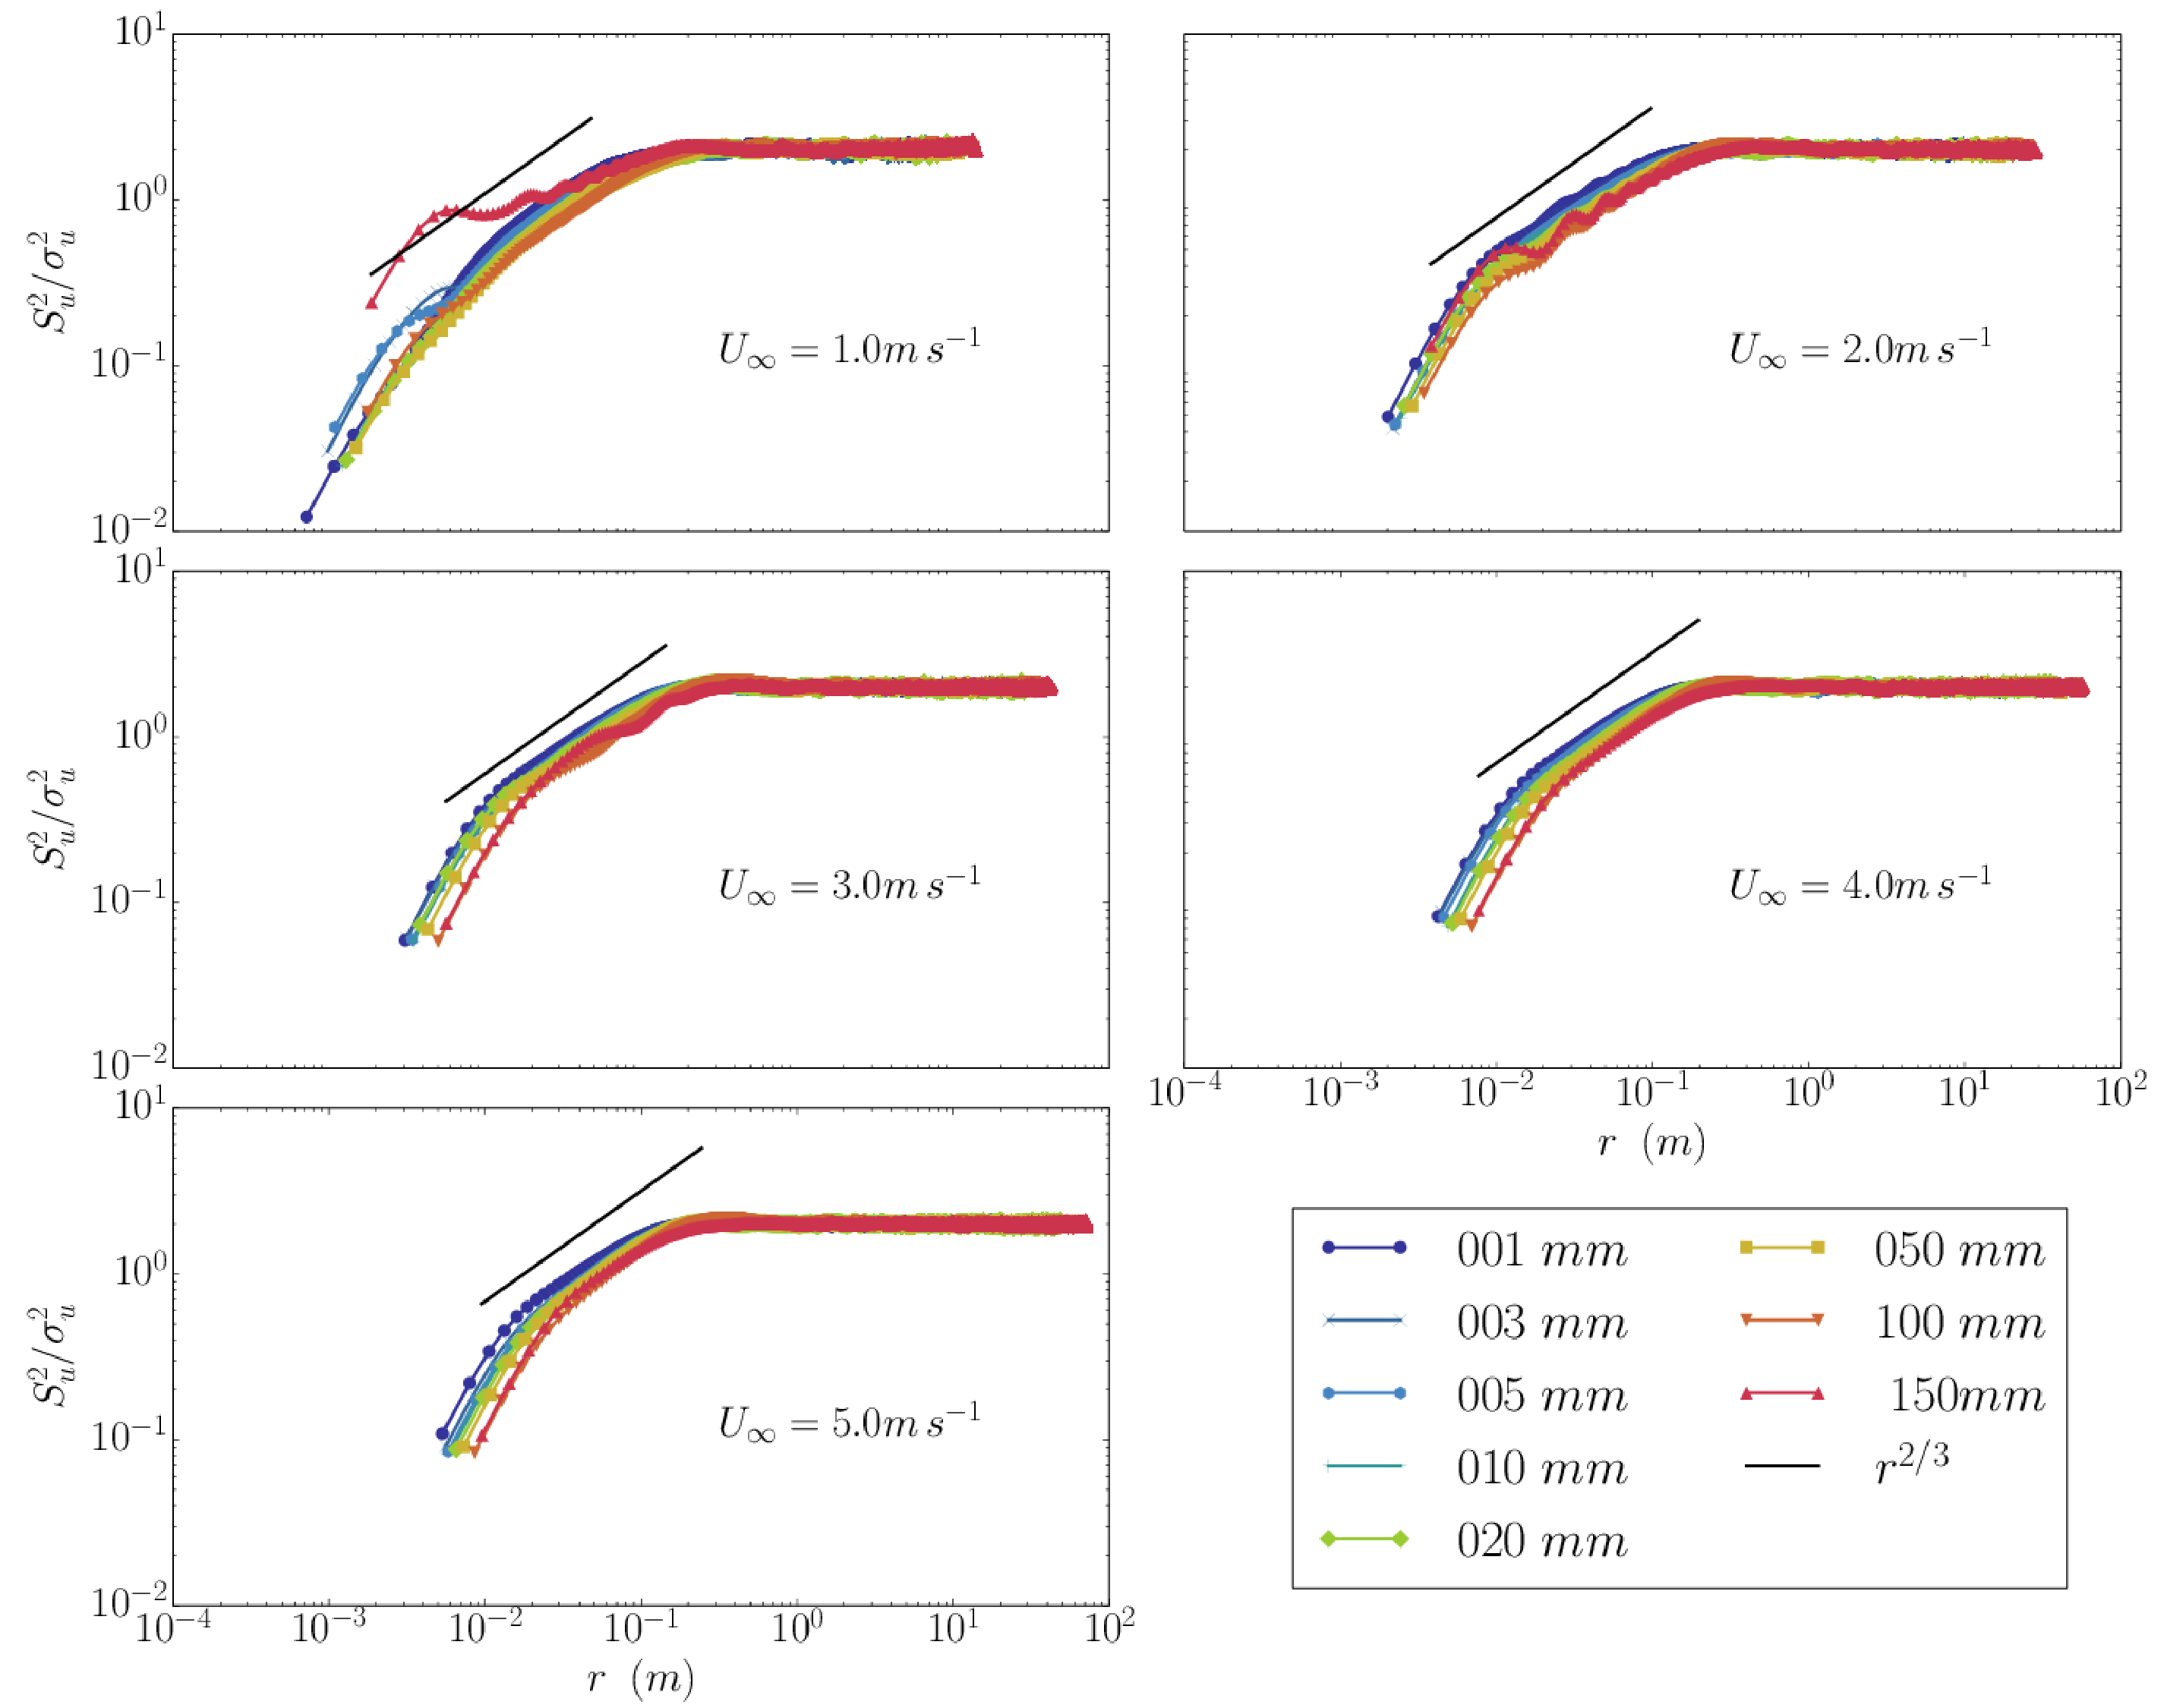
\includegraphics[width=0.6\textwidth]{figuras/estrutura_com.pdf}
		\caption{\label{exepretex3} Um exemplo de utilização do ambiente ``grafico''.}
		\fonte{Próprio autor.}
	    \end{grafico}
         \end{verbatim}
         
	    \begin{grafico}[ht]
	\caption{\label{exepretex3}Um exemplo de utilização do ambiente ``grafico''.}
             \centering
		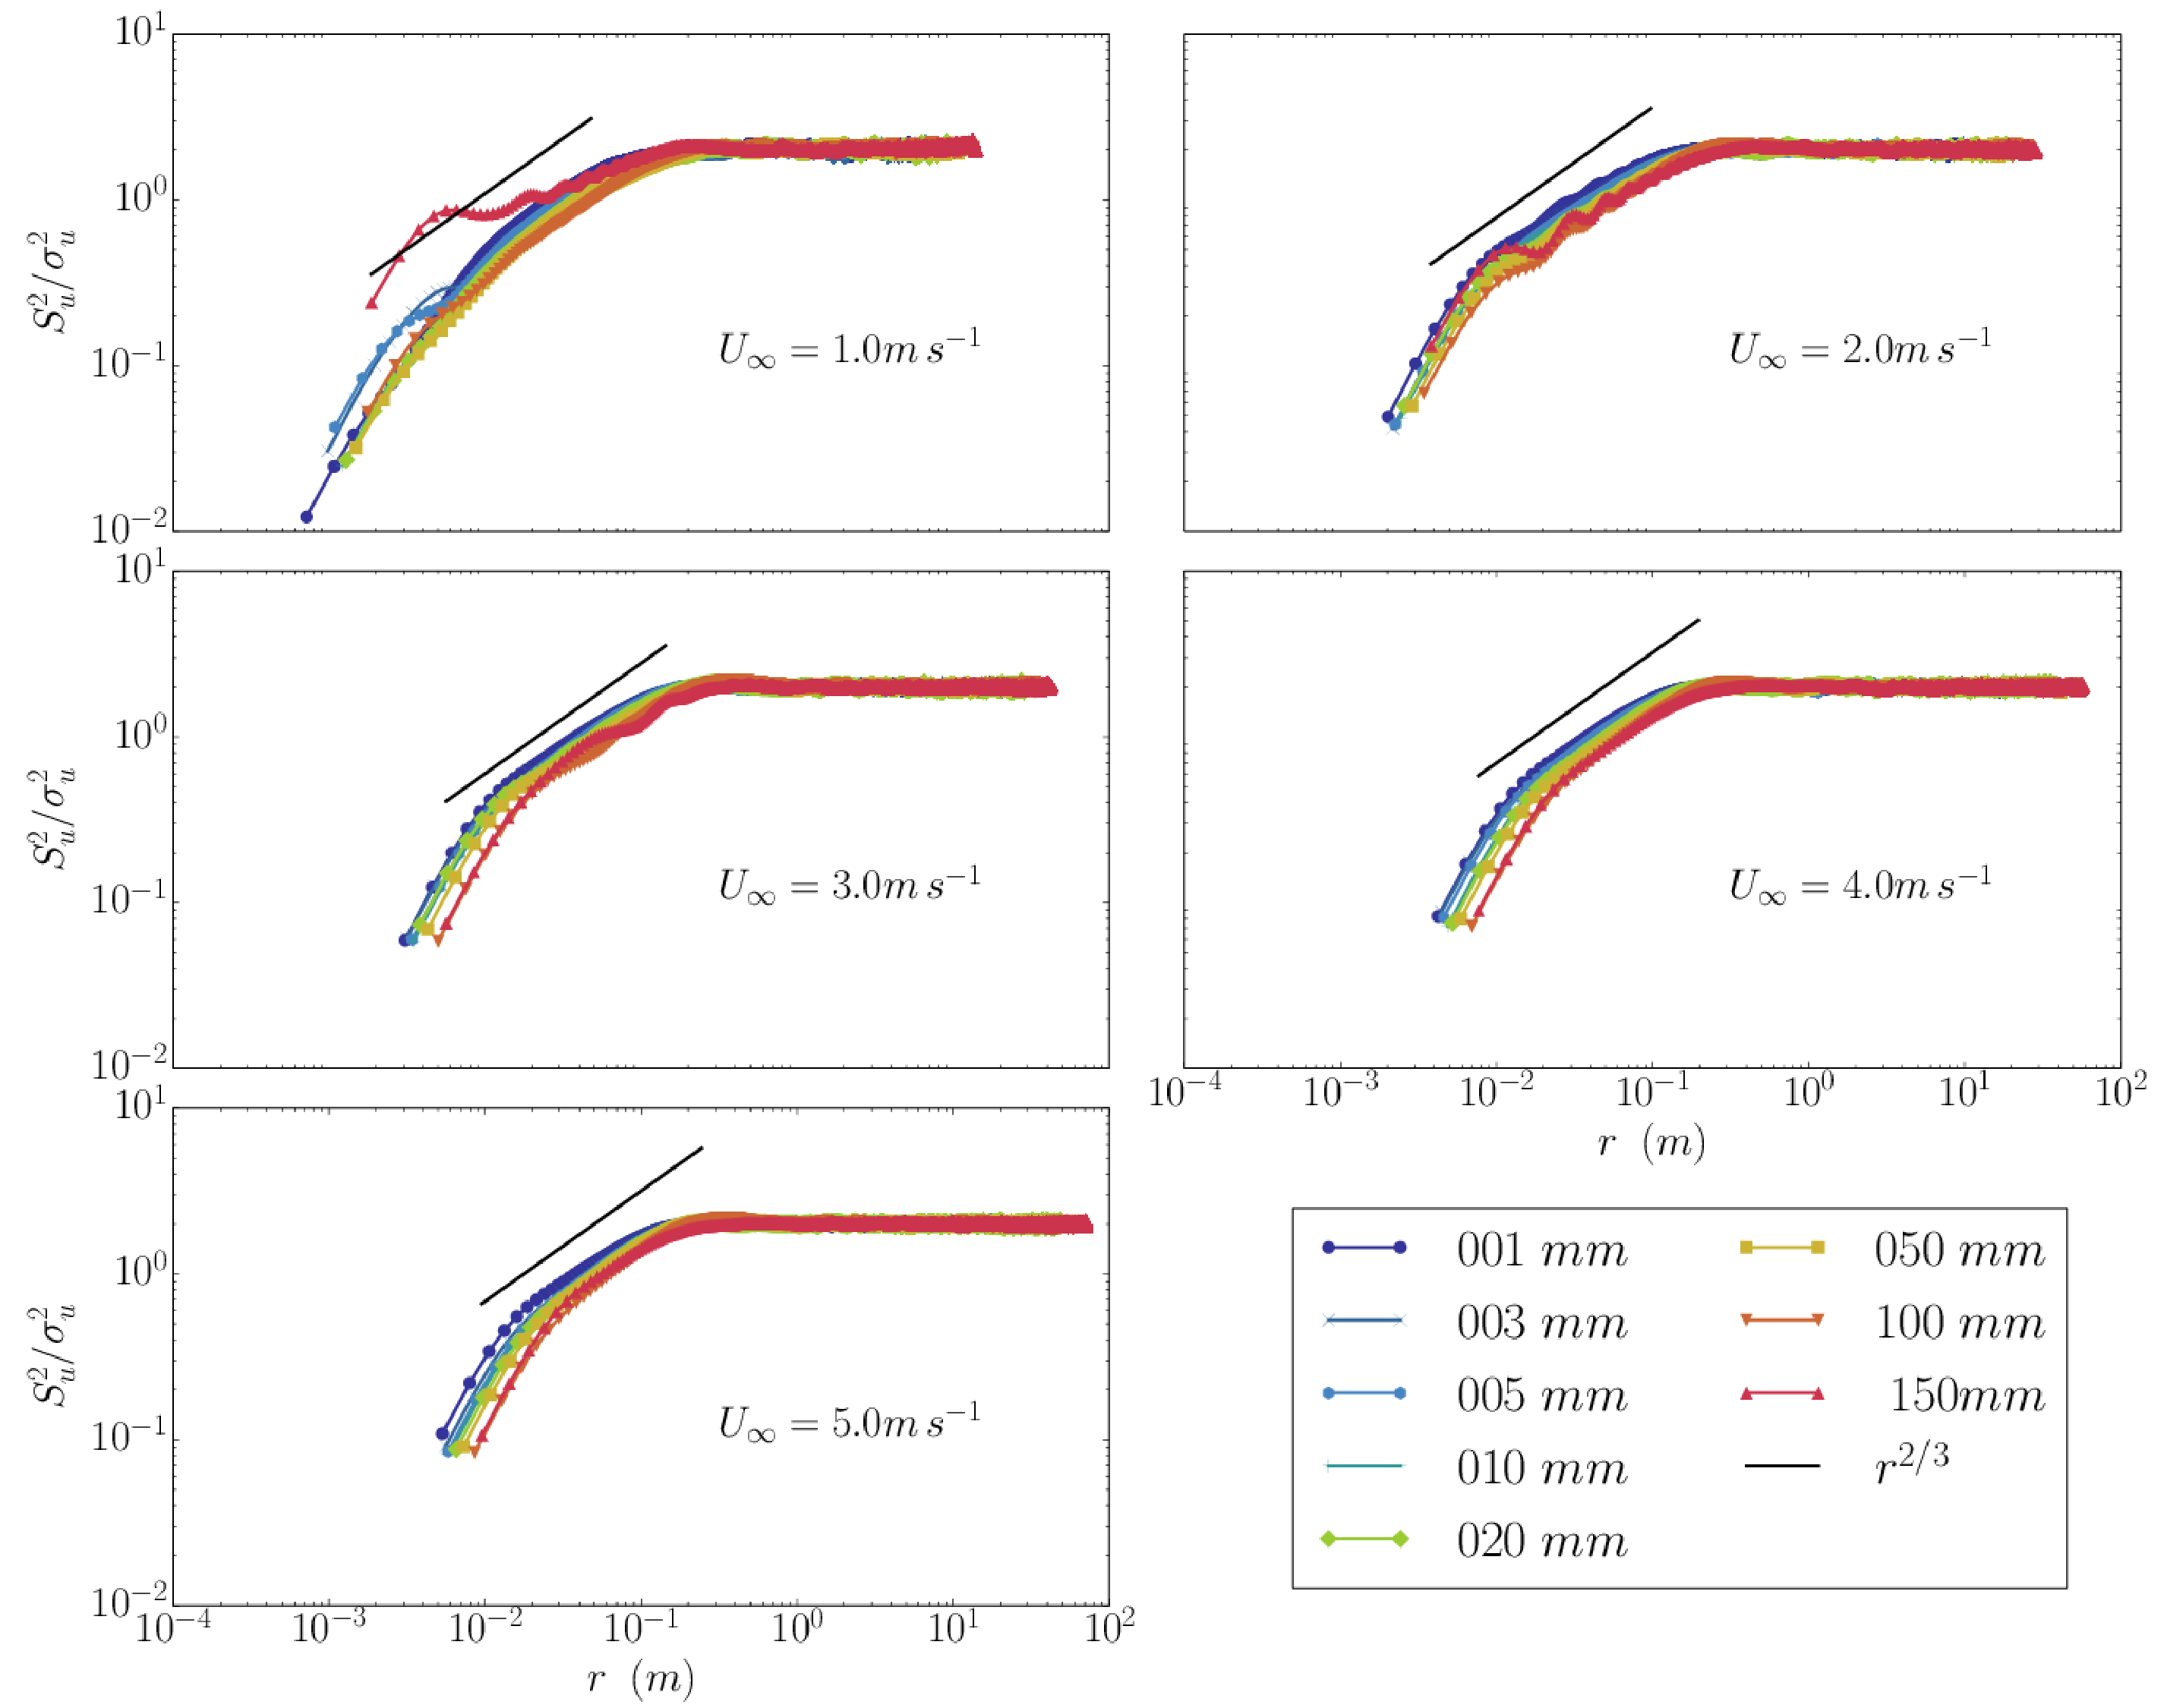
\includegraphics[width=0.6\textwidth]{figuras/estrutura_com.pdf}
		\fonte{Próprio autor.}
	    \end{grafico}
         
\chapter{Conclusão}

	\par Conclusão do trabalho.
	\lipsum[1-5]


	
	
% % % % % % % % % % % % % % % % % % % % % % % % % % % % % % % % % % % % % % 
% % % % % % % % % % % % FIM DAS PAGINAS TEXTUAIS % % % % % % % % % % % % % % 
% % % % % % % % % % % % % % % % % % % % % % % % % % % % % % % % % % % % % % 



% % % % % % % % % % % % % % % % % % % % % % % % % % % % % % % % % % % % % % 	
% % % % % % % % % % % % % BIBLIOGRAFIA  % % % % % % % % % % % % % % % % % % 
% % % % % % % % % % % % % % % % % % % % % % % % % % % % % % % % % % % % % % 	

\bibliografia{referencias}  %%%%% BIBLIOGRAFIA -> INCLUIR NAS CHAVES O NOME DO ARQUIVO *.BIB	
	
	
	
% % % % % % % % % % % % % % % % % % % % % % % % % % % % % % % % % % % % % 	
% % % % % % % % % % % % % APENDICES % % % % % % % % % % % % % % % % % % %
% % % % % % % % % % % % % % % % % % % % % % % % % % % % % % % % % % % % % 	
	\apendice %%%% TEXTOS A PARIR DESTE PONTO SERAO CONSIDERADOS APENDICES

\chapter{Demonstração de algo}
        \par Algo como apêndice.  
         \lipsum[2-10]

          
% % % % % % % % % % % % % % % % % % % % % % % % % % % % % % % % % % % % % % 	
% % % % % % % % % % % % % % % ANEXOS  % % % % % % % % % % % % % % % % % % % 
% % % % % % % % % % % % % % % % % % % % % % % % % % % % % % % % % % % % % % 	
        \anexo    %%%% TEXTOS A PARIR DESTE PONTO SERAO CONSIDERADOS ANEXOS
        
\chapter{Algo interessante que alguém fez}
         \par Algo como anexo.
         \lipsum[2-10]
                  
        \begin{grafico}[ht]
     	    \caption{\label{exepretex2}Orientações para a lombada do trabalho.}
	    \centering
	    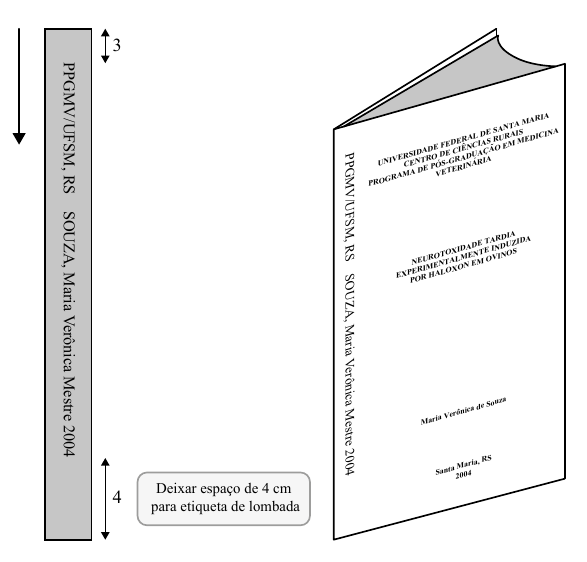
\includegraphics[width=0.6\textwidth]{figuras/lombada.png}
            \fonte{Adaptado de \citeonline{man:MDTUFSM2015}.}
         \end{grafico}         
         
         \lipsum[2-10]

      
         
\end{document}
